%===================================== CHAPTER 6 Design and architecture =================================

\chapter{Design and architecture}

To get a brief overview of the complete product and its required parts the design and architecture is presented in this chapter. It is not meant to give a complete understanding, but rather an overview on how the different parts of the product work together to give a good user experience.

\section{Architecture}

The overall architectural design of the system was made to achieve a rough mapping of what needed to be done in terms of actual programing. The architecture focuses heavily on interactions between the different instances in the systems without going into the specific details on how this is done. To illustrate the architecture two different views were created. One showing only the components, with another showing the processes in the different components. The overall system structure can be seen in \textbf{Fig \ref{Fig:system_structure}}, this shows the four different components and how they interact. In \textbf{Fig \ref{Fig:architecture}} a diagram showing the architecture with processes can be found. As seen in the legend, the square boxes represents individual components or processes. The boxes with oval corners represents compound processes or larger parts. These are mainly shown because they give an overview over which processes belong to and will be performed by which part of the system. Double lined boxes are external sources that provide an API. Lastly, arrows indicate information flow.

\begin{figure}[h!]
	\centering
	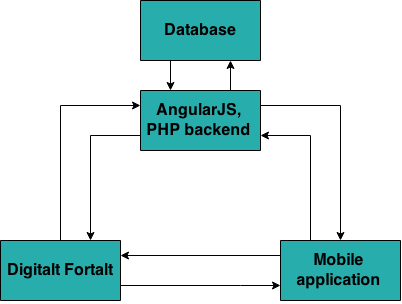
\includegraphics[width=0.5\textwidth]{fig/system_structure}
	\caption{Diagram of the overall system structure for this project.}
	\label{Fig:system_structure}
\end{figure}

It is a difficult task to model a whole system in an accurate way, and while the architecture diagram shows an overlook, it can not give much insight into the complexity of each process. This is further complicated by the fact that in the startup phase of the project there are a great number of unknowns. Both complexity and requirements are subject to change. As such, the diagram should only be used as a guide for understanding the composition of the complete system.

\begin{figure}[h!]
	\centering
	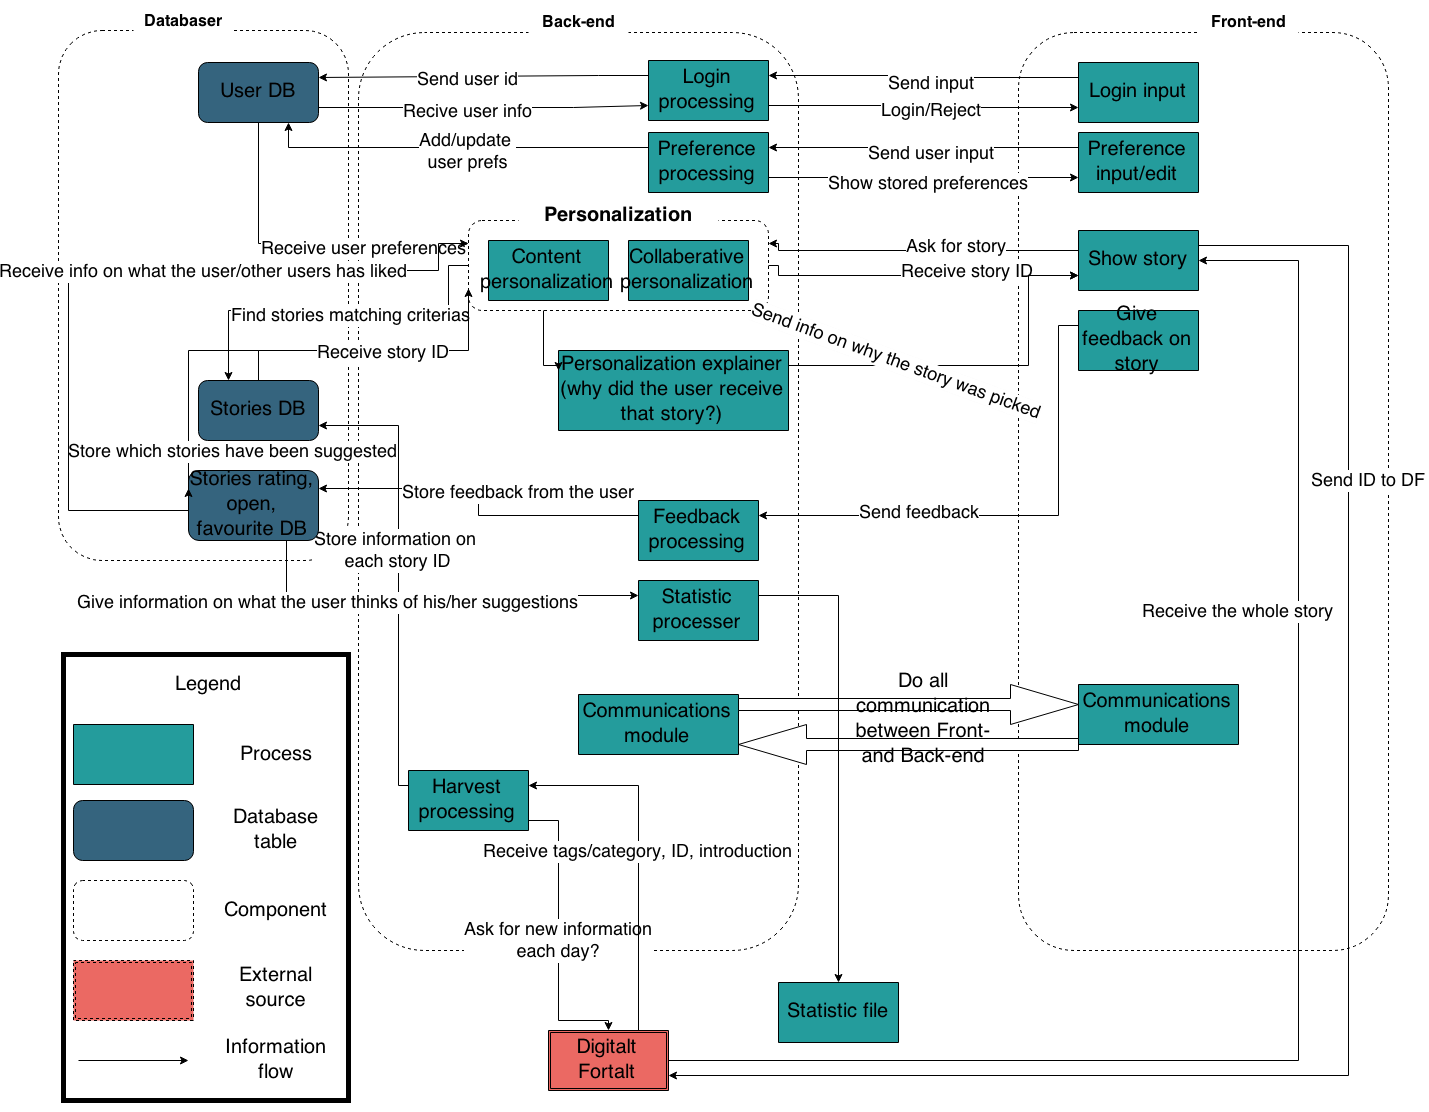
\includegraphics[width=\textwidth]{fig/architecture}
	\caption{Diagram of the architecture for this project.}
	\label{Fig:architecture}
\end{figure}

\section{Database design}
\label{sec:database_design}

The database was designed with the goal of facilitating the recommendation of stories to users. The data model underpinning the database is visualized in the ER-diagram in \textbf{Fig \ref{Fig:er_diagram}}. User and story are the central entities in this diagram, since the goal of the application is to connect users to stories. Both of these entities has a number of attributes describing the entity. The central relationship in the diagram is the recommendation-relationship, where a user and a story is connected. This connection is described by some additional attributes, such as rating, tag and state. \newline

To make the right connections between user and story, some attributes describing the user and the stories are necessary to store in the database. For instance, in order to make recommendations based on nine predefined categories, every story is mapped from subcategories gathered from Digitalt fortalt to one or more of the nine categories (see \textbf{Section \ref{sec:categorymapping}} category mapping). A user is connected to one or more of these categories by the setting of personal preferences. In addition, the database stores information about the changing state of recommended stories in order to make better recommendations. \newline

Another goal of this project is to provide some research data to the customer (see requirement RXX in appendix XX). To do this, some data about the use of the application is stored. This include registering what actions are taken during a user session. The state entity records changes in the state of stories connected to a user. For research purposes the customer also wished to know the relationship between satisfaction of a story (i.e the rating) and the media format contained in the story.

\begin{figure}[h!]
	\centering
	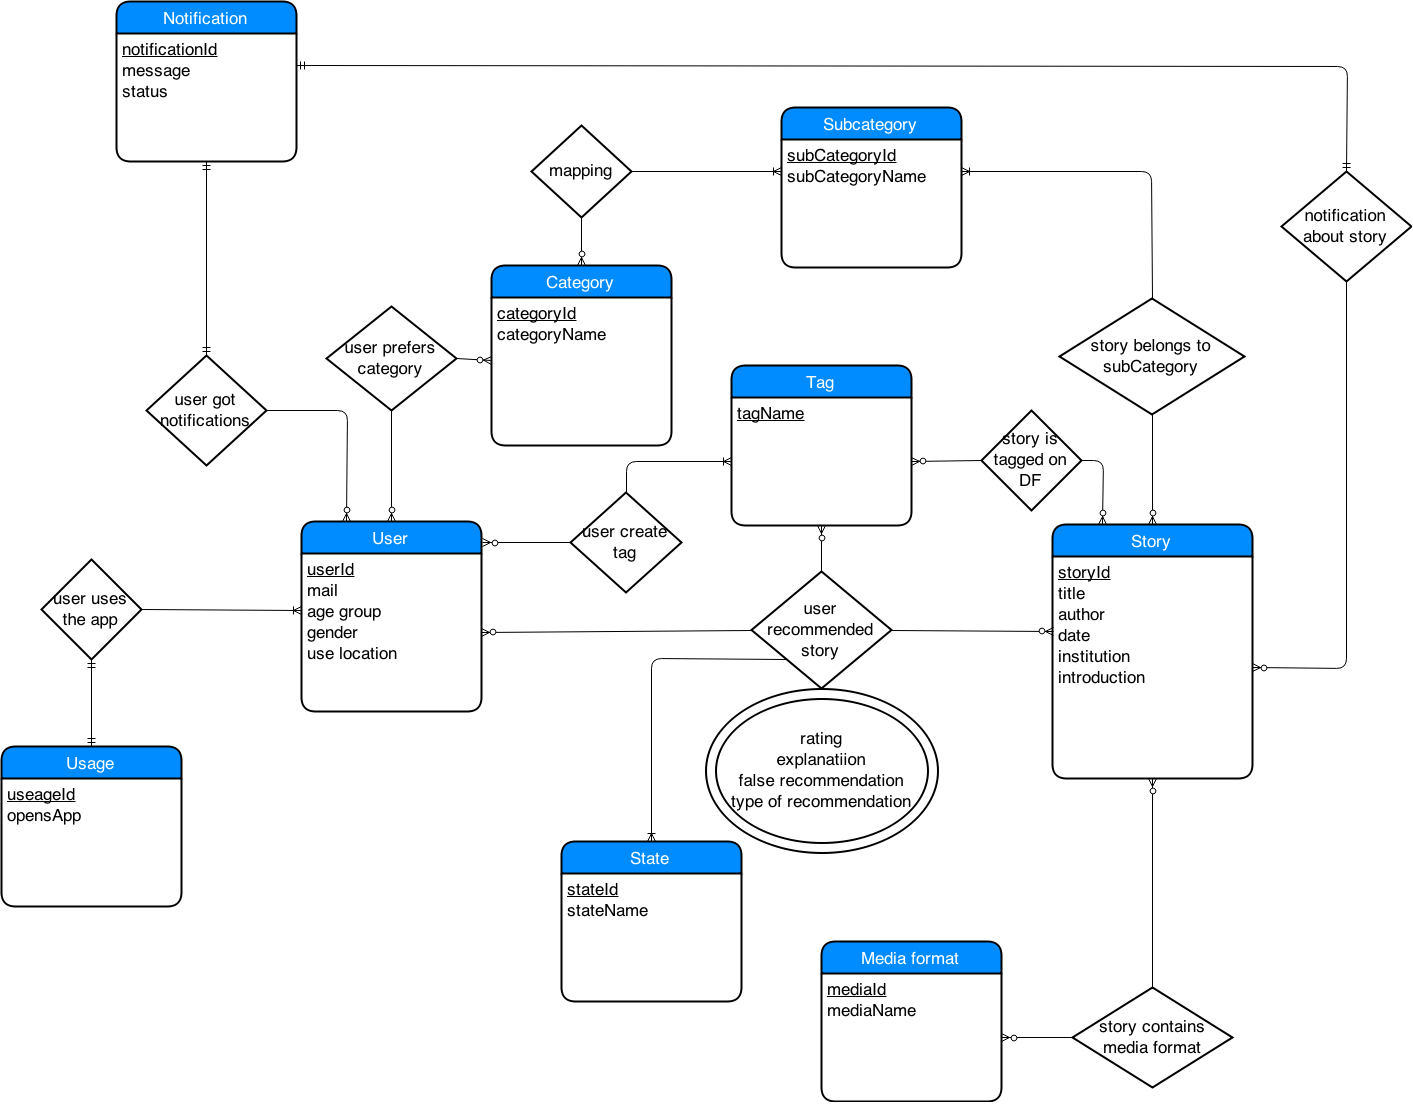
\includegraphics[width=\textwidth]{fig/er_diagram}
	\caption{ER-diagram showing the data model.}
	\label{Fig:er_diagram}
\end{figure}

In mapping the ER-diagram to a relational database the algorithm in [AS2, p.270-278] has been used. To ensure a good database design, four informal guidelines in [AS2, p. 487-497] have also been used. These guidelines are:

\begin{enumerate}
\item Making sure that the semantics of the attributes is clear in the schema\newline 
	This means that a relation schema (table) in the database corresponds to a entity type or a relationship type. The relational database used in this project follows this guideline by making a table for each entity and each relationship in the ER-diagram. The n-ary relationship “user recommend story” is split into tables according to the mapping algorithm.
\item Reducing the redundant information in tuples\newline
	This means that the tables should contain no insertion, deletion or modification anomalies. Our database is designed to avoid redundant information, so that modification of one attribute only have to be performed in one tuple in one relation schema. This results in quite a few tables, but maintains a consistent database.
\item Reducing the NULL values in tuples\newline
	Some of the tables in our database has the potential for NULL values. For instance, a user may access the application without entering an email address, which means that the user table could be filled with NULL values in the mail-column. An alternative solution would be to to create a user-mail table, which contain only a userId and the email address for those users who actually have entered a email address. The story table also has the potential for NULL values, for instance if a story lacks a connection to an institution.\newline
	
	Some of the problems associated with NULL values such as the use of aggregate operations and the multiple possible interpretations of what the NULL represents does not apply to our tables. Alternative solutions has not been employed because guideline 1 has taken priority. Story and user are the most important entities in our data model and should not be divided among too many tables since that makes retrieving complete information about them harder. 
\item Disallowing the possibility of generating spurious tuples \newline
	Means that tables should be joined on attributes that are appropriately related, that is primary keys and foreign keys. This guideline is followed in the database design in this project. 
\end{enumerate}

\section{User interface}

The user interface design was an essential part of the project, as the customer prioritized usability over all other nonfunctional requirements. The design thus went through many iterations by working on a prototype and continually getting feedback from customer and user tests. This feedback loop was important as the customer did not have clear requirements to the application from the beginning, and making everything easy to understand for the user was also challenging.  Balsamiq was first used to create a basic wireframe, but as it’s functionality was limited the next iteration of the design was made using Proto.io. This made it possible to receive better feedback on the flow of the app and not just the views individually. \newline

The following \textbf{Fig \ref{Fig:flow_diagram}} explains the overall flow between all the different views in the application. The blue boxes represent views, while the white ones represent modals placed on top of the view the user came from. The text of the arrows explains what the user clicked in the view the arrow comes from, and the arrow points to which view this action leads to.  The functionality of the more complex views will then be explained in further detail.

\begin{figure}[h!]
	\centering
	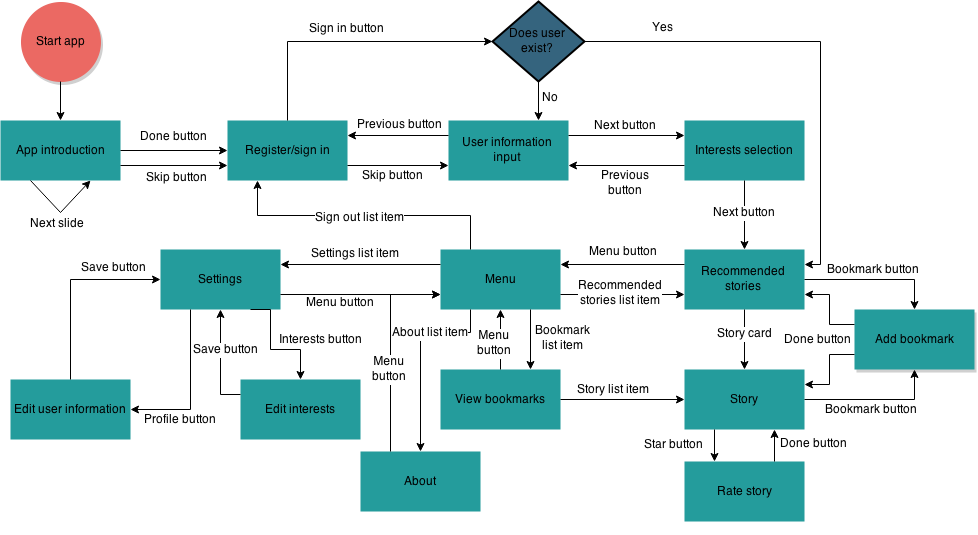
\includegraphics[width=\textwidth]{fig/flow_diagram}
	\caption{Diagram of the flow between views in the user interface.}
	\label{Fig:flow_diagram}
\end{figure}


Recommendation view\newline
This view displays the stories that should be the most relevant to the user. The user can browse them by swiping through them or by clicking the left and right arrows. When tapping on a card the detailed view of the story will be displayed. The “X” in the right corner of each card is used to reject the story, which takes it out of the list of the current recommendations and makes that kind of stories less likely to appear in the future. The bookmark icon in the top bar opens a modal for adding a bookmark. 

\begin{figure}[h!]
	\centering
	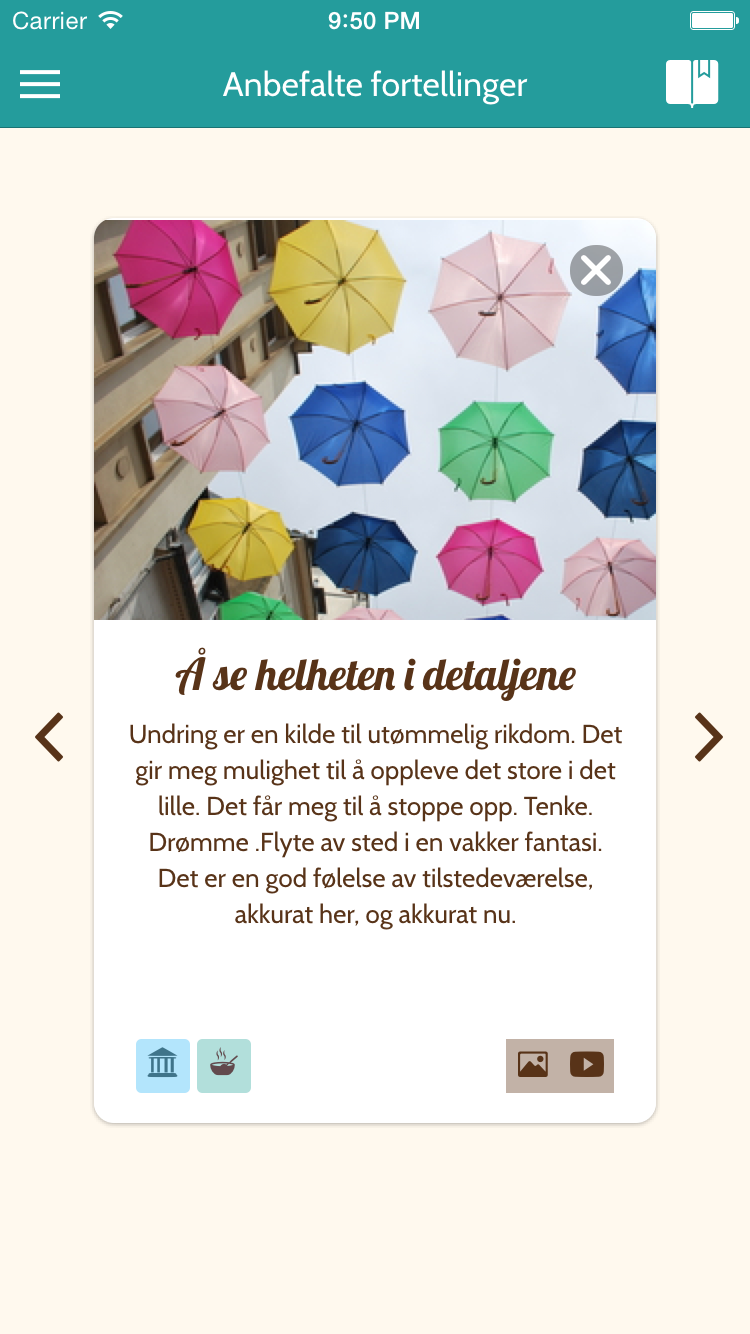
\includegraphics[width=0.5\textwidth]{fig/recommendation_view}
	\caption{Recommendation view}
	\label{Fig:recommendation_view}
\end{figure}

Story view\newline
This view displays the chosen story in detail. There is a box which displays the media files associated with the story. The tabs above it will depend on which media types the story contains. Videos will be displayed by default if there are any, as they can be a major component of the story which should not be hidden in another tab. When tapping on a video or image it will be displayed in fullscreen mode. The user can give feedback on the story either by tapping the stars on the bottom part of the view, or by tapping the star icon in the top bar which will open up a modal. The modal will ask the user to rate the story, and the user can exit it by tapping “Ferdig” or by tapping outside of the modal. Tapping the bookmark icon will make the same modal as in the recommendation view appear.

\begin{figure}[h!]
	\centering
	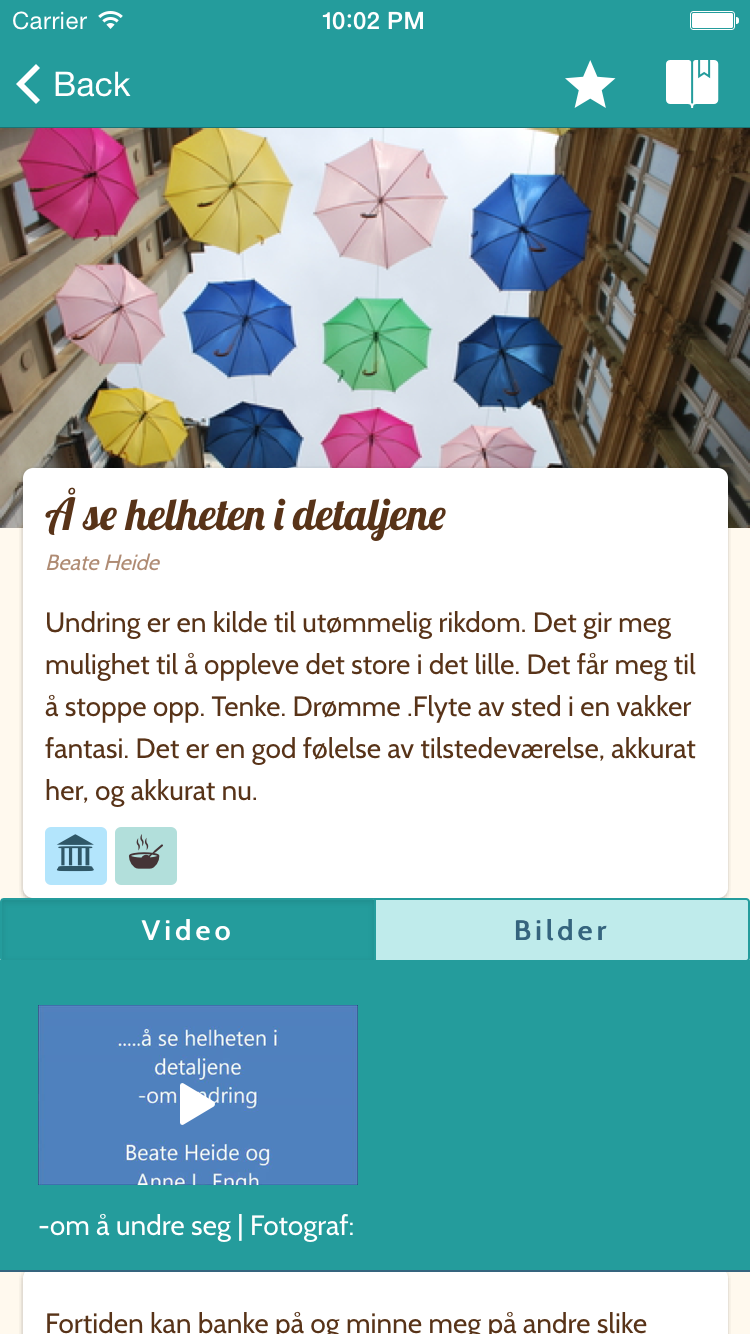
\includegraphics[width=0.5\textwidth]{fig/story_view}
	\caption{Story view}
	\label{Fig:story_view}
\end{figure}

TODO: Screenshots and explanations of other views

\section{Category mapping} 
\label{sec:categorymapping}

There are 31 subcategories presented at Digitalt fortalt. Each story can have 0 to 31 subcategories attached to it. To achieve a content based filtering the user has to select some interest categories. To make it easier for the user, these subcategories are divided into nine main interests categories. Some of these categories of interest were already predefined in [EHW1], while the rest was changed according to discussions with the customer. The subcategories were put into the category interest field that fit them best, with some subcategories being in several category interests. In \textbf{Table \ref{Tab:categorymapping}} this mapping is illustrated. It is obvious that some category interests will have more stories, however, subcategories such as literature contain more stories than most others. In such a way, it was intended to create nine category interests that contain roughly the same amount of stories. Even distribution of stories into category interests was intended, however, when a subset of stories was chosen this intention did not hold true as can be seen in chapter XX. Furthermore, the category interests needed to be distinct while still encompassing all the subcategories. 

\begin{table}[!h]
	\begin{center}
		\begin{tabular}{ | p{5cm} | p{12cm}|}
			\hline
			\textbf{Archeology} & Arkeologi og forminne \\ \hline
			\textbf{Architecture} & Arkitektur \\ \hline
			\textbf{Art and design} & Bildekunst, dans, design og formgjeving, film, fotografi, media, teater \\ \hline
			\textbf{History} & Historie, historie og geografi, kulturminne, sjøfart og kystkultur, språkhistorie \\ \hline
			\textbf{Local traditions and food} & Bunader og folkedrakter, dans, fiske og fiskeindustri, fleirkultur og minoritetar, Hordaland, kultur og samfunn, kulturminne, musikk, Rallarvegen, samer, sjøfart og kystkultur, språk, tradisjons- mat og drikke \\ \hline
			\textbf{Literature } & Litteratur, teikneseriar \\ \hline
			\textbf{Music} & Musikk \\ \hline
			\textbf{Nature and adventure} & Fiske og fiskeindustri, naturhistorie, sport og friluftsliv \\ \hline
			\textbf{Science and technology} & Fiske og fiskeindustri, fotografi, "kjøretøy, bil og motor, veitransport", media, "natur, teknikk og næring", "teknikk, industri og bergverk", skip- og båtbygging \\ \hline
		\end{tabular}
	\end{center}
	\caption{Category mapping performed to facilitate, and simplify content based filtering. Each category is assigned to one or more interests.}
	\label{Tab:categorymapping}
\end{table}

\section{Reuse of code}

Reusing written code can be a great help to quickly have progress when programming.  To investigate possibilities of this, the code from stedr was reviewed. However, since stedr used a different framework on the front end and java as the server language reusing code proved difficult. Therefore, the code written was developed without relying on previous work.

\subsection{Digitalt museum’s application programming interface}
\label{subsec:api}

All content related to stories displayed in the application was collected from Digitalt fortalt. Initially, to achieve better results when testing the personalization algorithms, the stories collected are limited to the areas Nord-Trøndelag and Sør-Trøndelag. The API [HM1] used to retrieve stories belongs to Digitalt museum. This API enables search through data from Digitalt museum, displaying pictures and provides access to an XML representation of available objects.\newline

Digitalt fortalt is established on the same technical platform as Digitalt museum [HM2]. This makes the integration better between the two and the remaining services in Norvegiana. Norvegiana is a datamodel, database and a web service with the purpose of making cultural heritage information more accessible [HM3]. Example services available in Norvegiana are Digitalt museum, Digitalt fortalt, Arkivportalen and Musikkarkiv. 

\cleardoublepage